%\documentclass[tikz,convert={density=800,outext=.png},border=5pt]{standalone}
\documentclass[tikz, border=5pt]{standalone}

\usepackage[utf8]{inputenc}					% Выбор языка и кодировки
\usepackage{amsmath} % nice math symbols
     

\usepackage{tikz}
\usetikzlibrary{shapes,positioning,calc,patterns,decorations.pathreplacing}

\newcommand{\situation}[3]{
	\node[draw, circle, fill=white, scale=1.5] (sit_#1) at (#2pt,#3pt) {};
}
\begin{document}
	
	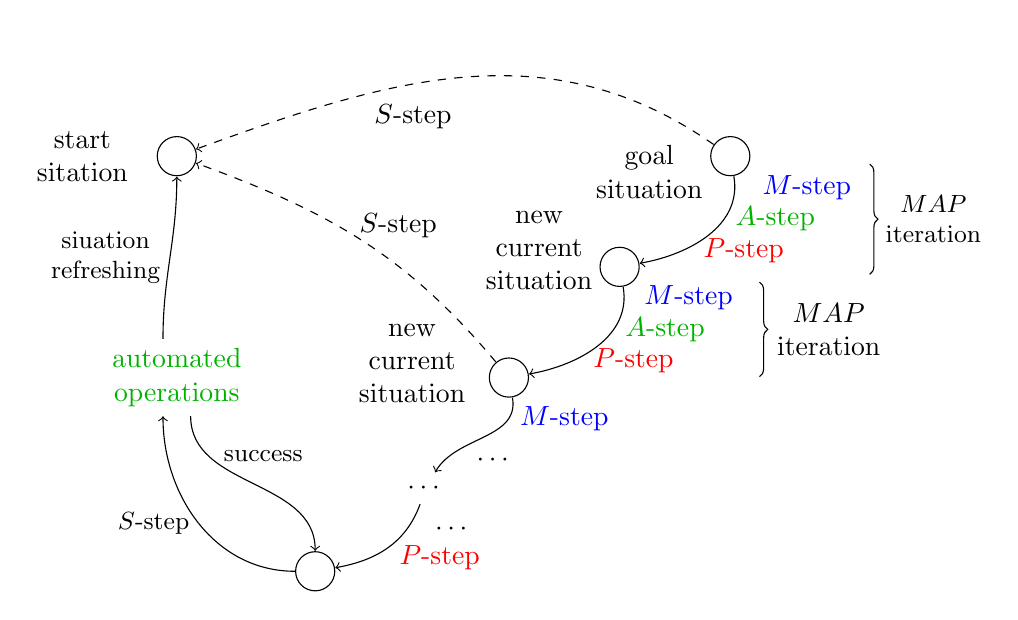
\begin{tikzpicture}
		\situation{st}{0}{0};
		\node[align=center] at (-1.2,0) {start\\sitation};
		\situation{end}{200}{0};
		\node[align=center] at (6,-0.2) {goal\\situation};
		
		
		\situation{1}{160}{-40};
		\situation{2}{120}{-80};
		\node (all) at (90pt,-120pt) {$\cdots$};
		\situation{3}{50}{-150};
		
		\draw[->] (sit_end) to[out=-80,in=10] (sit_1);
		\draw[->] (sit_1) to[out=-80,in=10] (sit_2);
		\draw[->] (all) to[out=-110,in=10] (sit_3);
		\draw[->,dashed] (sit_2) to[out=130,in=-20] (sit_st);
		\draw[->] (sit_2) to[out=-80,in=60] (all);
		
		\node[align=center, color=blue] at (8,-0.4) {$M$-step};
		\node[align=center, color=green!70!black] at (7.6,-0.8) {$A$-step};
		\node[align=center, color=red] at (7.2,-1.2) {$P$-step};
		\draw [decorate,decoration={brace,amplitude=3pt,mirror}]
		(8.8,-1.5) -- (8.8,-0.1) node[align=center,midway,font=\small,xshift=23pt] {$MAP$\\iteration};
		\node[align=center] at (4.6,-1.2) {new\\current\\situation};
		
		\node[align=center, color=blue] at (6.5,-1.8) {$M$-step};
		\node[align=center, color=green!70!black] at (6.2,-2.2) {$A$-step};
		\node[align=center, color=red] at (5.8,-2.6) {$P$-step};
		\draw [decorate,decoration={brace,amplitude=3pt,mirror}]
		(7.4,-2.8) -- (7.4,-1.6) node[align=center,midway,xshift=25pt] {$MAP$\\iteration};		
		\node[align=center] at (85pt,-75pt) {new\\current\\situation};

		\node[align=center, color=blue] at (140pt,-95pt) {$M$-step};
		\node[align=center] at (115pt,-110pt) {$\cdots$};

		\node[align=center] at (100pt,-135pt) {$\cdots$};
		\node[align=center, color=red] at (95pt,-145pt) {$P$-step};
		
		\node[align=center] at (80pt,-25pt) {$S$-step};

		
		\node[align=center, text=green!70!black] (ppo) at (0pt,-80pt) {automated\\operations};
		\draw[->] (sit_3) to[out=-180, in = -90] node[font=\small,left]{$S$-step} ([xshift=-5pt]ppo.south);

		\draw[->] ([xshift=5pt]ppo.south) to[out=-90, in = 90] node[font=\small,right,yshift=10pt,xshift=-14pt] {success} (sit_3);
		
		\draw[->] ([xshift=-5pt]ppo.north) to[out=90,in=-90] node[align=center,left, font=\small]{siuation\\refreshing} (sit_st);
		
		\draw[->,dashed] (sit_end) to[out=145, in = 20] (sit_st);
		\node[align=center] at (3,0.5) {$S$-step};
	\end{tikzpicture}


\end{document}